The {\bf shuffled complex evolution} (SCE) \cite{duan1992effective}
is a population
based evolutionary optimization algorithm that regards a natural 
evolution happening simultaneously in $N$ independent communities (or {\bf complexes}).

Initialy $N*M$ individuals are randomly taken from the feasible solution space and
sorted according to their fitness.
Subsequently a {\bf shuffling} process places the \nth{1} in the first complex,
the \nth{2} in second complex, individual N\ts{th} goes to N\ts{th} complex,
individual $M+1$ goes back to the first complex, etc.
\vspace*{-20pt}
\begin{center}
\noindent\begin{tabular}{@{\hspace{0.0em}}c@{\hspace{1.0em}}c@{\hspace{0.0em}}}
\hspace{-3mm}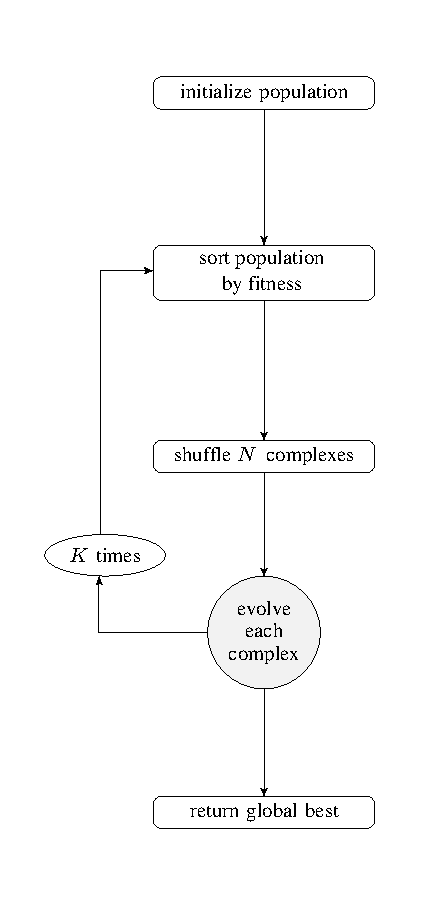
\includegraphics[width=0.46\linewidth]{imgs/flow1a} &
\hspace{-3mm}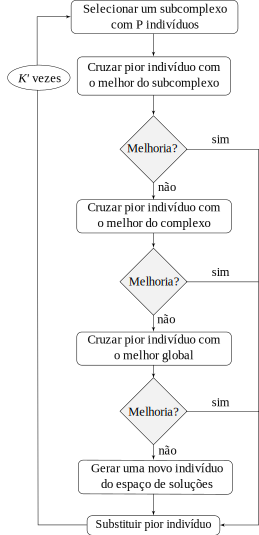
\includegraphics[width=0.46\linewidth]{imgs/flow2} \\
{\scriptsize The SCE algorithm.} & {\scriptsize Evolving stage.}
\end{tabular}
\end{center}
The next step after shuffling the complexes is to evolve each each of then through
a fixed amount of {\it (a)} $K'$ steps.
In each step {\it (b)} a {\bf subcomplex} of $P$ individuals is selected from the
complex, prioritizing those with better fitness.

The worst individual from the  subcomplex is identified to
be replaced by a new one generated by {\it (c)} its crossing 
with best individual of the subcomplex.

If the new solution has not improved {\it (d)} the best individual
of the {\bf complex} is considered for crossing and latter the {\it (e)} best one  
of whole {\bf population}.
If all the crossing steps couldn't improve the worst individual,
it is {\it (f)} replaced by a {\bf new random} solution.
